\documentclass[8pt]{extarticle}
\usepackage[margin=0.48in,top=0.42in,bottom=0.35in]{geometry}
\usepackage{graphicx,amsmath,amssymb,xcolor,enumitem,booktabs}
\usepackage[hidelinks]{hyperref}
\usepackage{helvet}
\renewcommand{\familydefault}{\sfdefault}

\setlist[itemize]{leftmargin=0.95em,topsep=0.5pt,itemsep=0.4pt,parsep=0pt}
\setlist[itemize,2]{leftmargin=0.95em,topsep=0.3pt,itemsep=0.2pt}
\setlength{\parindent}{0pt}
\usepackage{titlesec}
\titleformat{\section}{\bfseries\small}{\thesection.}{0.35em}{}
\titlespacing*{\section}{0pt}{3.5pt}{1.5pt}
\definecolor{acc}{HTML}{2d6a9f}
\newcommand{\hl}[1]{\textcolor{acc}{\textbf{#1}}}
\newcommand{\B}[1]{\textbf{#1}}
\setkeys{Gin}{width=0.985\textwidth}
\pagestyle{empty}

\begin{document}

{\large\bfseries What is in \texttt{embeddings.npz}?}\hfill
{\footnotesize Aviral Garg \;$\cdot$\; Forgis screening task \;$\cdot$\; 10 Oct 2026}\\[1pt]
{\footnotesize Every number here comes out of \texttt{code/analyze.py} (numpy/scipy/torch, no sklearn, seed 0,
about 4 minutes on CPU). Raw values are in \texttt{out/results.json}.}
\vspace{1.5pt}\hrule\vspace{1pt}

\section{Identification}

\B{Given:} \texttt{T} $(2500,512)$ f32, \texttt{I} $(2500,512)$ f32, \texttt{Y} $(2500,)$ i64. No other metadata.

\begin{itemize}
\item \B{\texttt{Y} is a class label:} 31 distinct values in $[1,34]$, 31--33 absent $\Rightarrow$ \hl{a subset of a
      34-class dataset}. 49--150 samples/class; majority class 6.0\%.
\item \B{Not $\ell_2$-normalised:} $\|\texttt{T}\|=9.06{\pm}0.86$, $\|\texttt{I}\|=10.19{\pm}0.46$. Raw encoder
      output, taken before any normalisation layer.
\item \B{Two different encoders:} per-dim variance correlation \hl{0.0017}, mean per-dim correlation 0.18, and
      only 4 of 512 dims reach $|r|>0.5$. They share no basis.
\item \B{\texttt{T}'s inputs repeat exactly, \texttt{I}'s never do:} \texttt{T} 2075/2500 unique (173 duplicate
      groups, max multiplicity 30), \texttt{I} 2500/2500. \hl{98.8\% of duplicate groups sit inside one class.}
      Note 83\% of \texttt{T} rows are still unique, so this is a pool with class-confined repeats rather than
      one string per class.
\item \B{Row order carries nothing:} $\cos(\texttt{I}_i,\texttt{I}_{i+1})=0.6579$ against $0.6581$ for a random
      pair, and the same at lags 2, 5, 10 and 50. \texttt{Y} has 2416 runs in 2500 rows.
\end{itemize}

\B{Hypothesis: a CLIP-style dual encoder, with \texttt{T}=text, \texttt{I}=image and \texttt{Y}=class.}
\begin{itemize}
\item \emph{For:} $D{=}512$ is CLIP ViT-B/32's shared width for both towers; the vectors are unnormalised,
      as a dump taken before the $\ell_2$ layer would be; two towers explain the disjoint bases; repeated
      captions explain \texttt{T}'s duplicates; and the mean-offset (\S4) matches CLIP's documented gap.
\item \emph{Against / open:} paired similarity barely exceeds same-class similarity (\S4), so the row pairing is
      \emph{class}-level; and 34 classes on their own weren't enough for me to pin down the source dataset.
      \hl{I'm putting this forward as a hypothesis with its evidence, and nothing stronger.}
\item \emph{Decisive test, which needs the source data:} encode known image/caption pairs with ViT-B/32 and
      compare norms, gap and spectrum. I have not measured reference CLIP norms myself.
\end{itemize}

\B{It is not a HEPA dump.} HEPA (Petersen et al., arXiv:2605.11130) emits a $(h_t,h^*)$ pair per sample, so I
tested for that. Three checks, all of them negative:
\begin{itemize}
\item $D{=}512 \neq$ HEPA's $d{=}256$ (their \S3.1).
\item No temporal structure, but HEPA's pairs index $(t,\Delta t)$ over episodes.
\item HEPA's representations are \B{$\ell_2$-normalised onto the unit sphere} (their appendix A.2, and
      table 7: ``L1 on L2-normalised''), whereas $\|\texttt{T}\|=9.06$, $\|\texttt{I}\|=10.19$.
      \emph{I first used a SIGReg-distance test here; it does not discriminate, because HEPA applies SIGReg to
      the predictor output $\hat h$ and never to $h_t$ or $h^*$, so a genuine dump need not look isotropic.}
\end{itemize}

\section{Geometry: every rank estimate disagrees}
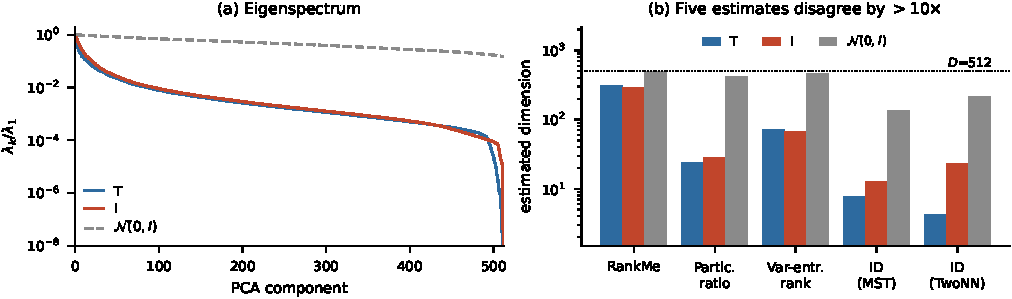
\includegraphics{figs/fig1_geometry.pdf}
\begin{itemize}
\item Strongly anisotropic: 90\% of variance needs 110 (\texttt{T}) / 93 (\texttt{I}) of 512 dims, after which
      the spectrum falls five orders of magnitude.
\item \hl{Five standard estimates span $>10\times$ on the same data} (\texttt{T}/\texttt{I}): RankMe 309/292,
      participation ratio 24/28, variance-entropy rank 71/66, MST-ID 7.7/12.9, TwoNN-ID 4.3/23.2, and
      \hl{they disagree on the ordering}: TwoNN puts \texttt{T}$\ll$\texttt{I}, RankMe puts
      \texttt{T}$>$\texttt{I}.
\item On an isotropic Gaussian control both ID estimators badly underestimate (136, 216 vs.\ a true 512), so at
      $N{=}2500,D{=}512$ \B{absolute ID values are untrustworthy}. I compare only within one estimator and name
      it every time.
\end{itemize}

\section{Isotropy, measured with HEPA's own regulariser}
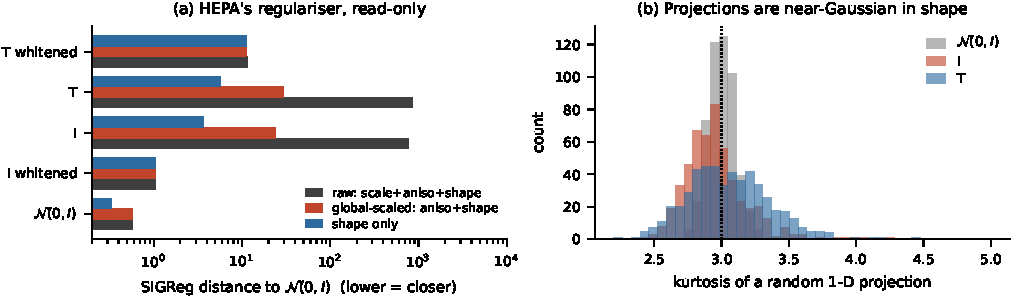
\includegraphics{figs/fig2_isotropy.pdf}
\begin{itemize}
\item \B{raw} is LeJEPA algorithm 1 verbatim (arXiv:2511.08544): random unit directions, \B{no centring, no
      rescaling}, Epps--Pulley with window $e^{-t^2/2}$, 17-knot trapezoid on $[-5,5]$. Only that line is the
      regulariser; the next three strip one factor each to locate the departure
      (\texttt{T} / \texttt{I} / $\mathcal{N}(0,I)$):
      \begin{itemize}
      \item raw \B{1091 / 1045 / 1.08} \;$\cdot$\; mean removed \B{860 / 781 / 0.57} \;$\cdot$\; $+$ one global
            rescale \B{29.8 / 23.9 / 0.57} \;$\cdot$\; $+$ per-projection standardised \B{5.7 / 3.7 / 0.33}.
      \end{itemize}
\item \hl{Almost all of the departure is scale and anisotropy; the shape is already near-Gaussian.} Mean
      projection variance 0.044 / 0.070 where SIGReg wants 1.0; projection kurtosis 3.06 / 2.95 against 3.00.
      This drives \S5.
\item \hl{Whitening \texttt{T} makes it worse:} shape-only 5.7$\to$11.4, kurtosis 3.06$\to$4.15, because
      whitening amplifies near-null directions into heavy tails. Whitening \texttt{I} behaves (1.04), so a
      blanket ``whiten first'' step isn't safe here.
\end{itemize}


\section{The modality gap is a rotation for class structure, not for instances}
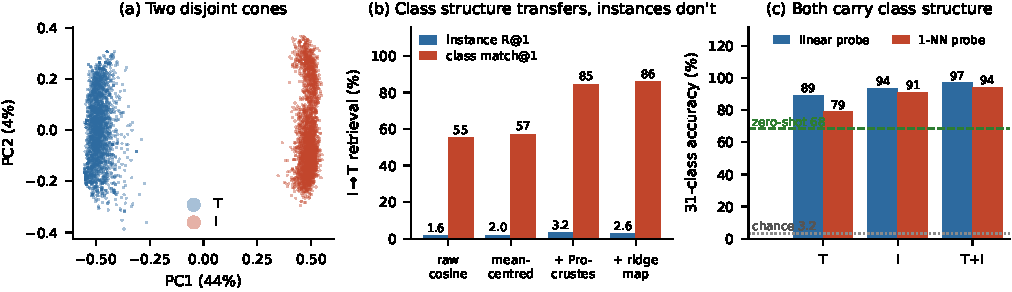
\includegraphics{figs/fig3_gap.pdf}
\begin{itemize}
\item \emph{Protocol:} centring, rotation and ridge map are fitted on the \B{2000 training rows}; retrieval is
      queried with the \B{500 held-out rows} against the full 2500-row gallery, so chance R@1 stays 0.04\%.
      \emph{An earlier version fitted and scored on all 2500 rows and read $1.6\%\!\to\!17.6\%$ at instance level
      against the $3.2\%$ below; class match moved far less (88.2\% vs 84.6\%), so the finding survives, narrowed.}
\item Disjoint clouds: $\cos(\overline{\texttt{T}},\overline{\texttt{I}})=0.319$,
      $\|\overline{\texttt{T}}-\overline{\texttt{I}}\|=0.97$ (normalised). PC1 alone separates them.
\item Raw cosine barely sees the pairing: paired 0.278, same-class 0.272, random 0.222. The 0.006 margin says the
      correspondence is \B{class}-level.
\item \hl{The rotation transfers at class level and barely at instance level} ($\texttt{I}\!\to\!\texttt{T}$,
      held-out): class match@1 \hl{55.4\%$\to$84.6\%}, but instance R@1 only 1.6\%$\to$\hl{3.2\%}
      ($80\times$ chance), R@5 7.2\%$\to$10.8\%. Mean-centring alone gives 2.0\% / 57.2\%.
      \hl{That split is the finding:} one orthogonal map recovers most of the class geometry across the gap and
      almost none of the instance correspondence, which is what the class-level pairing above predicts.
\item Zero-shot (held-out \texttt{I} classified by train-fitted class-mean \texttt{T} prototypes):
      68.4\% $\to$ \hl{89.0\%} after the same rotation; chance 3.2\%.
\item \B{Not a pure rotation:} an unconstrained ridge map edges class match (86.0\%) and loses instance R@1
      (2.6\%), with singular values far from flat (mean 0.22, s.d.\ 0.34).
\item Both carry class structure: linear probe 89.4 / 93.6 / 97.0\% and 1-NN 79.0 / 91.2 / 94.4\%
      (\texttt{T} / \texttt{I} / concat). \hl{The linear$-$kNN gap is $+10.4$ pts on \texttt{T} but $+2.4$ on
      \texttt{I}}, so \texttt{T}'s class information is linearly decodable while being less metrically organised.
      Repeated captions would do exactly that.
\end{itemize}

\section{Prediction in embedding space: cosine improves, nothing downstream does}
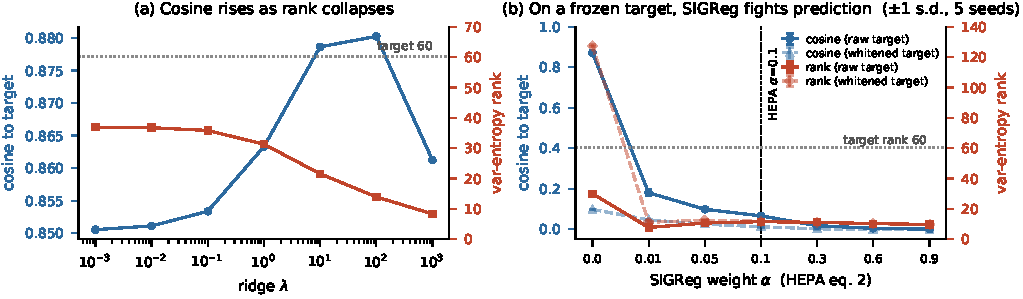
\includegraphics{figs/fig4_collapse.pdf}

\begin{itemize}
\item \emph{Setup:} the obvious JEPA experiment here. Context \texttt{T}, target \texttt{I}, predict in
      representation space. Held-out metrics; MLP results are mean\,$\pm$\,s.d.\ over \B{5 seeds}.
\item \hl{A ridge map looks better and better while collapsing.} Over $\lambda:10^{-3}\!\to\!10^{2}$, cosine
      \B{rises} 0.848$\to$0.882 and $R^2$ 0.13$\to$0.34, while the prediction's variance-entropy rank \B{falls}
      \hl{37.0$\to$14.2} against a target rank of 58.9. Had I reported cosine alone it would have hidden a
      $2.6\times$ rank collapse.
\item \hl{But rank does not predict the downstream number either.} Over that same range held-out retrieval is
      \B{flat} (R@1 8.0, 7.8, 7.8, 8.2, 8.4, 7.8\%) and only falls to 4.2\% at $\lambda{=}10^3$. So cosine
      improves monotonically while buying nothing downstream, and rank tracks the collapse but not the task.
      \B{Report all three.}
\item \B{SIGReg on the predictor does not fix it here.} 2-layer MLP under HEPA eq.~(2),
      $\mathcal{L}=(1-\alpha)\|\hat h - h^*\|_1+\alpha\mathcal{L}_{\text{SIGReg}}$: at $\alpha{=}0$,
      cosine $0.8716{\pm}0.0004$ / rank $30.0{\pm}0.1$; at HEPA's own $\alpha{=}0.1$, cosine \hl{$0.0609{\pm}0.0044$} / rank $11.9{\pm}0.2$.
      Every $\alpha\ge0.01$ destroys prediction, with seed spread far below the effect.
\item \B{Part of it is a scale conflict HEPA does not have.} HEPA trains ``L1 on L2-normalised'' representations
      (table 7), so both sides sit on the unit sphere; my frozen target has mean projection variance 0.070 while
      SIGReg wants 1.0. \B{Control:} against a whitened target (variance 1.000) that conflict is gone and
      prediction \emph{still} collapses (cosine $0.0985{\pm}0.0004$$\to$$0.0455{\pm}0.0034$ at $\alpha{=}0.01$; rank $128.0{\pm}0.7$$\to$$11.5{\pm}0.7$).
      So the remaining effect is about the target being \B{frozen}, not about its scale.
\item \hl{What this does and does not say about HEPA.} HEPA's target is never frozen: weight-shared and jointly
      trained (\S3.1), and \B{their appendix I.3 shows the method is robust to an EMA target instead}
      ($\tau{=}0.99$; joint wins 6/12, loses 4, ties 2, all within $\pm0.11$ h-AUROC), choosing joint training
      ``for its simplicity''. Both leave the target free to move toward the Gaussian SIGReg wants, and even
      $\tau{=}0.99$ is far more mobile than frozen. \hl{I measured the frozen-target regime, which neither
      setting in I.3 covers: there, no $\alpha$ bought both prediction and rank.} That gap is where my proposal
      starts.
\end{itemize}

\section{Caveats}
\begin{itemize}
\item \B{One 80/20 split throughout, seed 0: every fitted object in \S4 and \S5 is fitted on the 2000 training
      rows and scored on the 500 held out.} I don't resample it, so the split is an untested source of variance.
      MLP results are 5 seeds; the ridge sweep is exact. \S2--\S3 are descriptive statistics of all 2500 rows.
\item The CLIP identification is unconfirmed; the test is named in \S1.
\item The $\alpha$ sweep is one architecture at one budget (2-layer MLP, 200 epochs) on unnormalised targets.
      I'd stand behind the \emph{direction}, that SIGReg and the prediction term conflict on a frozen target,
      not the crossover point. I have not run HEPA itself. \B{Next:} resample the split, and find where the
      rotation's residual 15.4\% class error concentrates.
\end{itemize}

\end{document}
